\chapter{Evaluation}
\label{sec:evaluation}
\minitoc
\vspace*{1cm}



% NEW SECTION
\section{Methodology}
\label{sec:dockerStack}
For the evaluation of our tool, we opted for convenience to use Docker ~\cite{docker_def}, which we also discussed in Chapter ~\ref{sec:background}. Docker is a software that can package your application, its dependencies, system tools, system libraries and settings in a single comprehensive virtual container. This is because Docker is lightweight, portable and can improve application development and deployment considerably.

As we already mentioned in Chapter ~\ref{sec:architecture}, \pname{} is limited to web applications written in PHP. The most popular and widely deployed language for Web applications is undoubtedly PHP, powering more than 80\% of the top ten million websites and contributing to almost 140,000 open-source projects on GitHub ~\cite{githubinfo}. For this reasons, we opted to evaluate our tool on web-apps developed in PHP.

The first web application we test our tool on is WordPress. The WordPress CMS (Content Management System) ~\cite{docker_def} is one of the most popular open-source web application for managing and publishing content on the web, with nearly half of the top 1 million sites on the internet using it. While it powers more than a third of the web, what is more important about it, for us, is that it is written in PHP and widely used for building a variety of websites, ranging from simple blog spots to professional web sites. 

We tested our tool on second web application, Drupal CMS ~\cite{drupal}. Drupal is a free and open-source content-management framework written in PHP and distributed under the GNU General Public License. It is used as a back-end framework for at least 2.1\% of all Web sites worldwide ranging from personal blogs to corporate, political, and government sites.

Using Docker, and more specifically its docker-compose functionality, we where able to achieved a multi-container deployment through a single docker-compose YAML file for the following services:

\begin{itemize}
	\item {\tt NGINX }: An open-source, high-performance HTTP server which handles all the HTTP request made by \pname{} and forwarded to our WordPress or Drupal web applications.{~\cite{nginx}}
	\item {\tt WordPress and Drupal }: Both open-source CMS web application. Since having access to the code, we began by examining the existing system in terms of injecting bugs and performing our instrumentation.
	\item {\tt MariaDB }: A popular open source relational databases which we used to store and manipulate the WordPress data~\cite{mariadb}.
\end{itemize}

The official images for the above services can be found for free at Docker Hub. An illustration of the above infrastructure in the case of WordPress, can be viewed at Figure ~\ref{fig:multi-container}. Files and instructions for replicating this process can be found at the fuzzer's repository.

\begin{figure}[ht]
 \centering
 \captionsetup{justification=centering}
 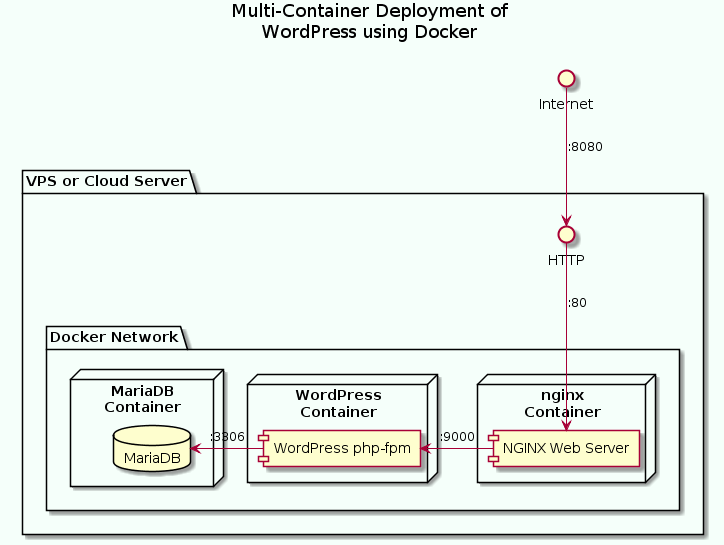
\includegraphics[width=\linewidth]{figures/multi-container.png}
 \caption{Evaluation followed the above Multi-Container Deployment of WordPress using Docker ~\cite{multi-container}.}
 \label{fig:multi-container}
\end{figure}

\section{Automated Vulnerability Addition}\label{sec:automated}
Evaluating fuzzing processes has proven to be a challenging task ~\cite{klees2018Evaluation}. Migrating known vulnerabilities to existing software, in order to test the capabilities of the fuzzer in finding bugs, can be a tedious process ~\cite{bug-reproduction}. Thus, for evaluating \pname{}, but also other fuzzers for web applications, an automated bug injection methodology, inspired by LAVA ~\cite{dolan2016lava} was used for automatically injecting bugs in web applications written in PHP. Injecting vulnerabilities in web code, again, is challenging, since important tools used for analysing native code and injecting vulnerabilities (e.g., taint-tracking and information-flow frameworks), are not available for web applications. To overcome this lack of available tools, the vulnerability injection methodology leverages the instrumentation infrastructure we use for building \pname{}, in the first place. The automated bug injection method is able to inject hundreds of common vulnerabilities such as Reflected Cross-Site Scripting in reasonable time. Details about the automated vulnerability addition, like the instrumentation, are out of the scopes of this thesis.

\section{Evaluation Details}
For the evaluation of \pname{}'s performance we used two Ubuntu 18.04 LTS Linux machines both possessing a quad-core Intel® Xeon® W-2104 Processor @3.20 GHz and 64GB of RAM. Targeted web applications consist of (a) an instrumented WordPress 5.5.1 with artificial bugs(b) a vanilla  WordPress 5.5.1 with artificial bugs, and (c) an instrumented Drupal 9.0.6. The term vanilla refers to web-apps in their original form, with no customizations or frameworks added to them. All artificial bugs where created with the automated vulnerability injection tool mentioned in  Section ~\ref{sec:automated}. Using this methodology, we managed to inject 150 identical Reflected Cross-Site Scripting bugs successfully in both the instrumented and vanilla versions of WordPress. Lastly, the Docker Stack of services described in Section ~\ref{sec:dockerStack} is deployed and running the web applications.